%%
%% Commands for TeXCount
%TC:macro \cite [option:text,text]
%TC:macro \citep [option:text,text]
%TC:macro \citet [option:text,text]
%TC:envir table 0 1
%TC:envir table* 0 1
%TC:envir tabular [ignore] word
%TC:envir displaymath 0 word
%TC:envir math 0 word
%TC:envir comment 0 0

%%
%% For anonymous submission (double-blind review), use:
\documentclass[sigconf,anonymous,review,9pt]{acmart}

%%
%% \BibTeX command to typeset BibTeX logo in the docs
\AtBeginDocument{%
  \providecommand\BibTeX{{%
    Bib\TeX}}}

%%
%% Rights management information - REMOVE/COMMENT OUT ALL FOR ANONYMOUS SUBMISSION
%% Restore these after acceptance for camera-ready version
%%
\setcopyright{acmlicensed}
\copyrightyear{2026}
\acmYear{2026}
\acmDOI{XXXXXXX.XXXXXXX}
\acmConference[DAC'26]{Design Automation Conference}{July 26--29, 2026}{Long Beach, CA, USA}
\acmISBN{978-1-4503-XXXX-X/26/07}

%%
%% Submission ID - Use if provided by conference
%%\acmSubmissionID{123-A56-BU3}

%%
%% Additional packages
\usepackage{amsmath,amssymb,amsfonts}
\usepackage{multirow}
\usepackage{algorithm}
\usepackage{algorithmic} 
%%
%% end of the preamble, start of the body of the document source.
\begin{document}

%%
%% The "title" command
\title{Energy-Guided Continuous Diffusion for Unsupervised Chip Placement}

%%
%% Author information
%% When using 'anonymous' option, this will be automatically hidden
\author{Ruogu Chen}
\affiliation{%
  \institution{University of Alberta}
  \department{Department of Electrical and Computer Engineering}
  \city{Edmonton}
  \state{AB}
  \country{Canada}
}
\email{ruogu@ualberta.ca}

\author{Jie Han}
\affiliation{%
  \institution{University of Alberta}
  \department{Department of Electrical and Computer Engineering}
  \city{Edmonton}
  \state{AB}
  \country{Canada}
}
\email{jhan8@ualberta.ca}

%%
%% The abstract
\begin{abstract}
Chip placement is a crucial process in integrated circuit design. The quality of the placement directly impacts performance, power consumption, and routability. Recent machine learning-based approaches have shown promising results but they also face significant limitations. Reinforcement learning (RL) methods suffer from poor generalization and require extensive retraining for each new circuit. Existing diffusion model-based methods are generalizable but lack explicit optimization objectives during the generation process. This article presents an energy-guided continuous diffusion model trained by using policy gradients. This method starts from random placements and iteratively refines them through a denoising process. This denoising process is guided by an energy function that represents the placement quality. The energy-guided diffusion approach not only enables parallel placement of all components but also requires no optimal placement examples for training. It enables efficient training on diverse synthetic data that covers most of the real chip data distributions. Therefore, the model learns general placement strategies that can be transferred to new designs without retraining. Experiments on standard benchmarks (ISPD 2005, ICCAD 2004) demonstrate that the proposed method achieves state-of-the-art placement quality with superior cross-circuit generalization.
\end{abstract}

%%
%% CCS concepts
% \begin{CCSXML}
% <ccs2012>
% <concept>
% <concept_id>10010147.10010178.10010179</concept_id>
% <concept_desc>Computing methodologies~Machine learning</concept_desc>
% <concept_significance>500</concept_significance>
% </concept>
% <concept>
% <concept_id>10010583.10010786</concept_id>
% <concept_desc>Hardware~Electronic design automation</concept_desc>
% <concept_significance>500</concept_significance>
% </concept>
% <concept>
% <concept_id>10010583.10010588.10010559</concept_id>
% <concept_desc>Hardware~Physical design (EDA)</concept_desc>
% <concept_significance>500</concept_significance>
% </concept>
% </ccs2012>
% \end{CCSXML}

% \ccsdesc[500]{Computing methodologies~Machine learning}
% \ccsdesc[500]{Hardware~Electronic design automation}
% \ccsdesc[500]{Hardware~Physical design (EDA)}

%%
%% Keywords
\keywords{Chip placement, diffusion models, reinforcement learning, proximal policy optimization, electronic design automation, denoising diffusion, macro placement, physical design}

%%
%% This command processes the author and affiliation and title
%% information and builds the first part of the formatted document.
\maketitle

\section{Introduction}

Chip placement is the process of determining the optimal physical locations of circuit components on a two-dimensional silicon canvas. The quality of the placement directly affects key design metrics such as wirelength, routability, power consumption, and timing performance. This process remains one of the most critical and computationally intensive steps in modern integrated circuit design~\cite{nam2005ispd2005, lin2019dreamplace}. 

Traditional analytical methods formulate placement as continuous optimization~\cite{lin2019dreamplace}, but it often converge to local optima due to the non-convex optimization landscape~\cite{cheng2024escaping, shi2024bboplace}. Machine learning-based approaches have shown promising results but face fundamental limitations: Reinforcement learning (RL) placement methods, such as CircuitTraining~\cite{mirhoseini2021graph}, exhibit poor generalization and require expensive retraining for each new circuit~\cite{kahng2023reevaluating, yue2022scalability}. In addition, by casting placement as a Markov Decision Process, sequential RL-based placements face challenges that the suboptimal placements during the early stage of the generation cannot be reverted~\cite{lee2024chip}. Recent diffusion-based approaches~\cite{lee2024chip} demonstrate improved generalization through zero-shot transfer to new circuits that never appeared in the training data. However, they rely on supervised learning from optimal placement examples, which are expensive to acquire through human experts or commercial Electronic Design Automation (EDA) tools. Additionally, existing diffusion-based methods apply guidance only during inference rather than training, limiting the model's ability to learn explicit optimization strategies~\cite{lee2024chip}.

We propose a continuous diffusion framework that addresses these limitations by leveraging energy-based guidance during training itself. This approach extends Scalable Discrete Diffusion Samplers (SDDS)~\cite{sanokowski2025scalable} from discrete combinatorial optimization to continuous chip placement. Unlike sequential RL methods that place components one at a time, the proposed diffusion approach performs parallel optimization over all components. Critically, energy is computed at every diffusion step rather than only at the final placement, providing dense feedback signals that significantly improve sample efficiency beyond standard policy-gradient diffusion methods. This approach enables unsupervised learning directly from the energy function without requiring optimal placement examples, allowing efficient training on diverse synthetic data. The main contributions are:
\begin{itemize}
\item We extend policy gradient-based diffusion training from discrete to continuous domains for chip placement, enabling unsupervised learning from energy functions without optimal placement examples. Unlike supervised diffusion methods that require costly ground-truth placements, this approach learns directly from placement quality metrics.
\item We introduce dense per-time step energy feedback that provides immediate gradient signals rather than propagating sparse terminal rewards across long trajectories. This reduces gradient variance by 3.2$\times$ compared to sparse-reward baselines.
\item We demonstrate zero-shot generalization from synthetic training data to real benchmarks (ISPD 2005, ICCAD 2004), achieving 3.7--5.6\% Half-perimeter wire length (HPWL) improvements over state-of-the-art supervised diffusion baselines without per-circuit retraining.
\end{itemize}

The remainder of this paper is organized as follows. Section~\ref{sec:related} reviews related work. Section~\ref{sec:preliminaries} introduces the preliminaries. Section~\ref{sec:method} presents the energy-guided continuous diffusion framework.
Section~\ref{sec:experiments} presents experimental results. Section~\ref{sec:discussion} concludes the paper and discusses future directions. The source code can be found here\footnote{\url{https://anonymous.4open.science/r/UCP}}

\section{Related Work}
\label{sec:related}

\textbf{Analytical Methods.} Traditional chip placement methods like DREAMPlace~\cite{lin2019dreamplace} formulate the problem as continuous optimization with GPU-accelerated differentiable engines. While achieving strong performance, they often converge to local optima due to the highly non-convex placement landscape~\cite{cheng2024escaping, shi2024bboplace} and require careful manual tuning that may not generalize well across designs.

\textbf{Reinforcement Learning Methods.} Google's CircuitTraining~\cite{mirhoseini2021graph} pioneered deep RL for chip placement but suffers from poor generalization requiring expensive per-circuit retraining~\cite{kahng2023reevaluating}, irreversible sequential placement decisions~\cite{lee2024chip}, and sparse reward credit assignment~\cite{lai2022maskplace}. While MaskPlace~\cite{lai2022maskplace}, ChiPFormer~\cite{lai2023chipformer}, and EfficientPlace~\cite{geng2024efficientplace} improve training efficiency, cross-circuit generalization remains unresolved.

\textbf{Diffusion Models.} Lee et al.~\cite{lee2024chip} demonstrated that diffusion models achieve competitive chip placement through zero-shot transfer by training on synthetic data using supervised learning from near-optimal placements, then applying guided sampling during inference.

\textbf{RL for Diffusion.} Recent work trains diffusion models with reinforcement learning, enabling optimization without optimal examples. Black et al.~\cite{black2024ddpo} fine-tuned text-to-image models via policy gradients. For combinatorial optimization, DiffUCO~\cite{sanokowski2024diffuco} and SDDS~\cite{sanokowski2025scalable} used energy-based guidance with PPO for discrete problems. Our work extends RL-based diffusion training to continuous chip placement, learning directly from placement quality metrics.


\section{Preliminaries}
\label{sec:preliminaries}

\subsection{Diffusion Models}
\label{subsec:diffusion_background}
Continuous diffusion models generate data by learning to reverse a gradual noising process~\cite{ho2020denoising, song2020score}. The forward diffusion process progressively corrupts data $\mathbf{x}_0$ by adding Gaussian noise over $T$ time steps. Starting from clean data at $t=0$, increasingly noisy states are obtained through:
\begin{equation}
\label{eq:forward_diffusion}
\mathbf{x}_t = \sqrt{1 - \beta_t} \cdot \mathbf{x}_{t-1} + \sqrt{\beta_t} \cdot \boldsymbol{\epsilon}, \quad \boldsymbol{\epsilon} \sim \mathcal{N}(0, \mathbf{I})
\end{equation}
where $\beta_t \in (0, 1)$ defines the noise schedule. A cosine schedule~\cite{nichol2021improved} is commonly used to control noise injection across time steps. At $t=T$, the data is corrupted to pure Gaussian noise.

Then the reverse process iteratively denoises from random noise back to clean data. In this denoising process, a neural network $q_\theta$ learns to predict the conditional distribution:
\begin{equation}
\label{eq:reverse_dist}
q_\theta(\mathbf{x}_{t-1}|\mathbf{x}_t, t) = \mathcal{N}(\boldsymbol{\mu}_\theta(\mathbf{x}_t, t), \boldsymbol{\sigma}^2_\theta(\mathbf{x}_t, t) \cdot \mathbf{I})
\end{equation}
This framework has achieved remarkable success in image generation~\cite{dhariwal2021diffusion}, audio synthesis~\cite{kong2021diffwave}, video generation~\cite{ho2022video}, and molecular conformation~\cite{xu2022geodiff}, demonstrating its versatility across diverse continuous domains.

\subsection{Policy Gradient Training}
\label{subsec:policy_gradient_background}
Traditional diffusion models are trained to match data distributions via maximum likelihood~\cite{ho2020denoising} or score matching~\cite{song2020score}. Although they enable high-quality result generations, these approaches typically require high volumes of high-quality examples from the target distribution. For chip placement, optimal placements require expensive commercial tools or human expertise, which is difficult to acquire or scale.

An alternative approach is to train diffusion models through \emph{policy gradients} from reinforcement learning (RL)~\cite{sutton2018reinforcement}, optimizing directly for solution quality without requiring optimal examples. This method treats the reverse diffusion process as a decision-making policy that iteratively refines the entire placement through denoising steps. In this view:
\begin{itemize}
\item The diffusion model $q_\theta(\mathbf{x}_{t-1}|\mathbf{x}_t, t)$ acts as a {policy} that samples the next state $\mathbf{x}_{t-1}$ given current state $\mathbf{x}_t$.
\item A complete diffusion trajectory $\mathbf{x}_{T:0} = (\mathbf{x}_T, \mathbf{x}_{T-1}, \ldots, \mathbf{x}_0)$ from noise to solution corresponds to an {episode}.
\item The final state $\mathbf{x}_0$ is evaluated by a {reward function} $R(\mathbf{x}_0)$ measuring solution quality.
\end{itemize}

The policy gradient theorem~\cite{sutton2018reinforcement} provides a way to compute gradients of the expected reward with respect to policy parameters $\theta$:
\begin{equation}
\label{eq:policy_gradient}
\nabla_\theta \mathbb{E}_{\mathbf{x}_{T:0} \sim q_\theta}[R(\mathbf{x}_0)] = \mathbb{E}_{\mathbf{x}_{T:0} \sim q_\theta}\left[\sum_{t=1}^{T} \nabla_\theta \log q_\theta(\mathbf{x}_{t-1}|\mathbf{x}_t, t) \cdot \hat{A}_t\right]
\end{equation}
where $\hat{A}_t$ is the {advantage function} quantifying how much better the sampled action at time step $t$ is compared to the expected value. This gradient can be estimated from sampled trajectories, enabling learning without supervised labels.

In practice, policy gradient optimization is performed using PPO~\cite{schulman2017proximal}, an on-policy RL algorithm that stabilizes training by limiting policy updates through a clipped objective. PPO uses Generalized Advantage Estimation (GAE)~\cite{schulman2015gae} to compute advantages $\hat{A}_t$ from temporal differences along the trajectory. This combination provides stable, sample-efficient learning for stochastic policies.

SDDS~\cite{sanokowski2025scalable} applies this policy gradient framework to train diffusion models for discrete combinatorial optimization problems such as the Traveling Salesman Problem (TSP) and Maximum Independent Set (MIS). SDDS operates on binary state spaces $\{0,1\}^N$ and it uses a sparse reward structure. It means that the reward function evaluates only the final solution $R(\mathbf{x}_0)$, providing no intermediate feedback during the diffusion trajectory.

This sparse reward structure leads to the credit assignment problem~\cite{sutton2018reinforcement}. This is a fundamental challenge in RL because it is difficult to determine which of the $T$ sequential decisions contributed to the final outcome. In the case of diffusion models, this single reward must be distributed backward across the entire trajectory through GAE's exponential decay mechanism $(\gamma\lambda)^l$. For structured problems like chip placement, where components interact through long-range nets spanning the circuit, this creates high-variance gradient estimates as the optimization signal becomes exponentially attenuated for early time steps~\cite{sutton2018reinforcement}.


\section{Methodology}
\label{sec:method}

\subsection{Problem Formulation}
\label{subsec:problem}

Chip placement is formulated as an energy minimization problem over continuous 2D coordinates. Given a netlist $\mathcal{G} = (\mathcal{V}, \mathcal{E})$ with $N$ components (macros and standard cells) and nets connecting them, the goal is to find positions $\mathbf{x} = \{(x_i, y_i)\}_{i=1}^N$ on a 2D canvas of dimensions $W \times H$ that minimize an energy function $E(\mathbf{x})$ while satisfying placement constraints. Following standard practice~\cite{lee2024chip}, all component positions and sizes are normalized to a $[-1, 1] \times [-1, 1]$ coordinate system (canvas center $c = (0, 0)$, half-width $L = 1$ in each dimension). This normalization enables training on diverse circuit sizes and simplifies the energy formulation.

To evaluate placement quality, two key metrics are used, following~\cite{lee2024chip}. First, the legality measures whether a placement satisfies physical constraints: no component overlaps, all components within canvas boundaries. Legality is defined as the ratio $A_u / A_s$ where $A_u$ is the area within the circuit boundary occupied by the union of all placed components, and $A_s$ is the sum of individual component areas. A legality score of 1 indicates that all constraints are satisfied. Second, HPWL serves as a proxy for chip performance by approximating routed wirelength. Our objective is therefore to generate legal placements ($A_u / A_s = 1$) with minimal HPWL.

The goal is to learn a conditional distribution $q_\theta(\mathbf{x}|\mathcal{G})$ that maps netlists to high-quality placements by minimizing expected energy:
\begin{equation}
\label{eq:learning_objective}
\theta^* = \arg\min_\theta \mathbb{E}_{\mathcal{G} \sim p(\mathcal{G})} \mathbb{E}_{\mathbf{x} \sim q_\theta(\cdot|\mathcal{G})} [E(\mathbf{x})]
\end{equation}

The energy function captures placement quality through three differentiable components:
\begin{equation}
\label{eq:energy}
E(\mathbf{x}) = E_{\text{wire}}(\mathbf{x}) + \lambda_{\text{overlap}} E_{\text{overlap}}(\mathbf{x}) + \lambda_{\text{bound}} E_{\text{bound}}(\mathbf{x})
\end{equation}

Following ChipDiffusion~\cite{lee2024chip}, the wirelength term computes HPWL for each net $e \in \mathcal{E}$:
\begin{equation}
\label{eq:hpwl}
E_{\text{wire}}(\mathbf{x}) = \sum_{e \in \mathcal{E}} \left[\max_{i \in e}(x_i) - \min_{i \in e}(x_i) + \max_{i \in e}(y_i) - \min_{i \in e}(y_i)\right]
\end{equation}

The overlap penalty penalizes pairwise component overlaps following ChipDiffusion~\cite{lee2024chip}:
\begin{equation}
\label{eq:overlap}
E_{\text{overlap}}(\mathbf{x}) = \sum_{i < j} \left[\min(0, d_{ij}(\mathbf{x}))\right]^2
\end{equation}
where $d_{ij}(\mathbf{x})$ is the signed distance between rectangular components $i$ and $j$. For axis-aligned rectangles with centers $(x_i, y_i)$, $(x_j, y_j)$ and half-sizes $(w_i/2, h_i/2)$, $(w_j/2, h_j/2)$:
\begin{equation}
\label{eq:signed_distance}
d_{ij}(\mathbf{x}) = \max\left(|x_i - x_j| - \frac{w_i + w_j}{2}, |y_i - y_j| - \frac{h_i + h_j}{2}\right)
\end{equation}
When components overlap, $d_{ij} < 0$ and the penalty is activated. When components do not overlap, $d_{ij} > 0$ and $\min(0, d_{ij}) = 0$, resulting in zero penalty. The squaring makes the penalty differentiable everywhere and emphasizes larger violations.

The boundary penalty enforces canvas constraints by penalizing components that extend outside the $[-1, 1] \times [-1, 1]$ canvas:
\begin{equation}
\label{eq:boundary}
E_{\text{bound}}(\mathbf{x}) = \sum_{i=1}^N \left[\max\left(0, |x_i| + \frac{w_i}{2} - 1\right)^2 + \max\left(0, |y_i| + \frac{h_i}{2} - 1\right)^2\right]
\end{equation}
For each component $i$, we compute how far each edge extends beyond the canvas boundary. The max function returns zero if the component is within bounds, and the violation distance otherwise. The squared penalty provides smooth gradients for optimization.

\begin{figure*}[t]
\centering
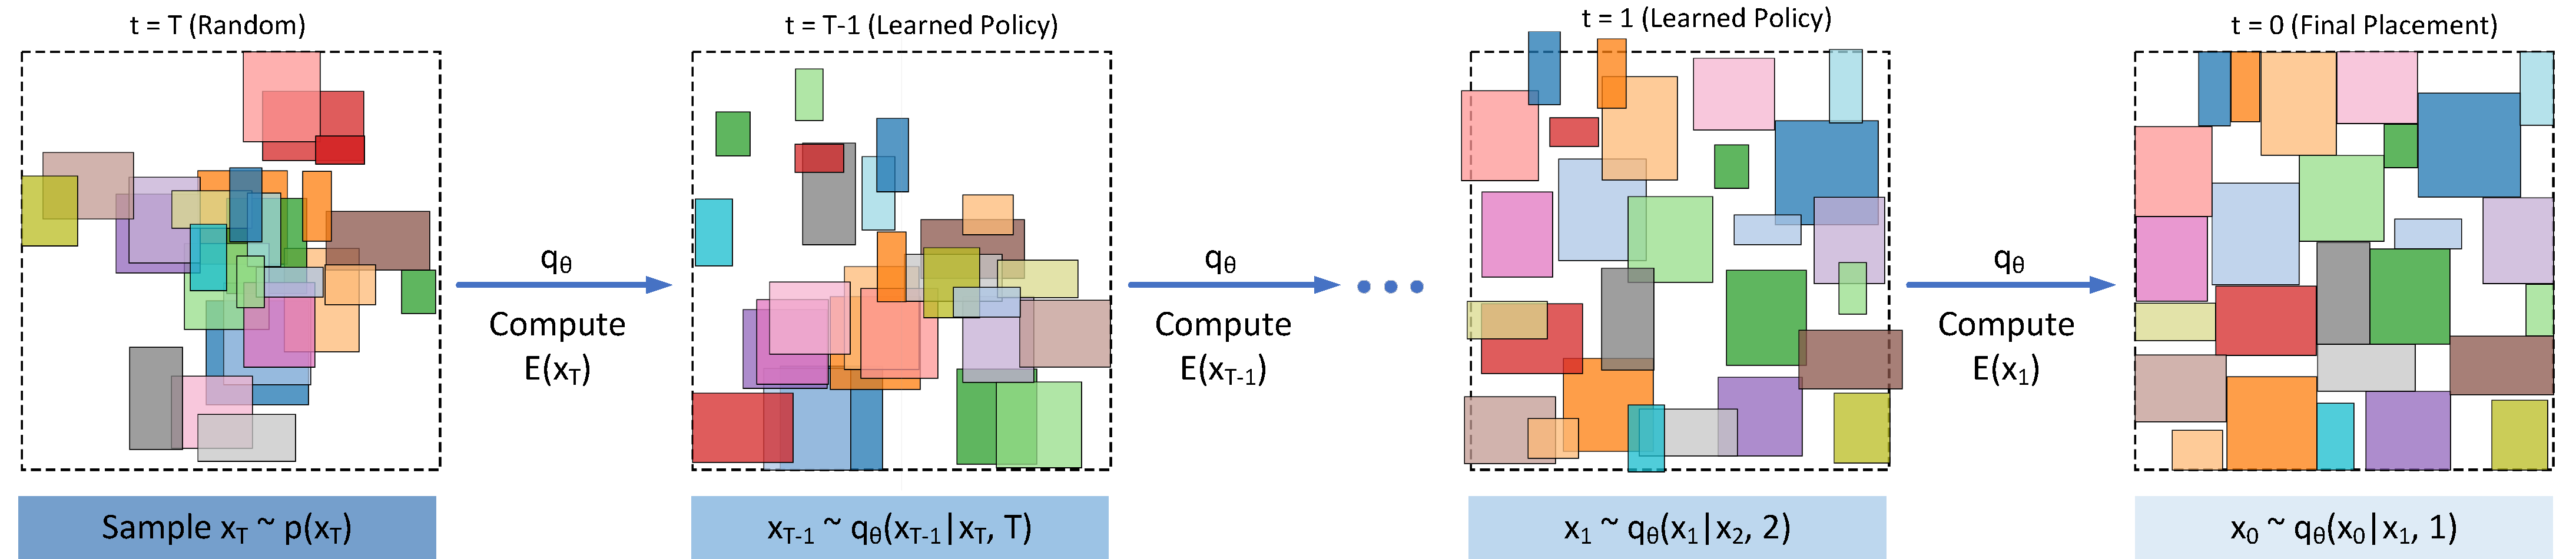
\includegraphics[width=\textwidth]{graphs/Diffusion Process.pdf}
\caption{The energy-guided reverse diffusion process: the learned policy $q_\theta$ progressively refines component positions from random noise ($t=T$) through intermediate states to final legal placement ($t=0$).}
\label{fig:energy_guided_diffusion}
\end{figure*}

\subsection{Training Method}
\label{subsec:dense_training}
We extend the SDDS policy gradient framework in two key ways. First, we adapt it from discrete binary state spaces $\{0,1\}^N$ to {continuous} 2D chip placement coordinates $\mathbf{x} \in \mathbb{R}^{2N}$. Second, we address the credit assignment problem by introducing dense energy feedback. The energy is computed at every diffusion time step rather than only after the final solution.

The policy gradient framework from Equation~\ref{eq:policy_gradient} and PPO algorithm apply directly to this continuous setting. However, unlike SDDS and similar policy-gradient methods~\cite{sanokowski2025scalable, mirhoseini2021graph} that use sparse terminal rewards $R(\mathbf{x}_0)$, we define per-step rewards that include the energy evaluated at the current state. For a trajectory $\mathbf{x}_{T:0} = (\mathbf{x}_T, \mathbf{x}_{T-1}, \ldots, \mathbf{x}_0)$ sampled from the reverse policy $q_\theta$, we define the per-step reward:
\begin{equation}
\label{eq:reward}
r_t(\mathbf{x}_t, \mathbf{x}_{t-1}) = -E(\mathbf{x}_t) + \alpha_{\text{noise}} \log p(\mathbf{x}_t|\mathbf{x}_{t-1}) + \alpha_{\text{ent}} \mathcal{H}(q_\theta(\mathbf{x}_{t-1}|\mathbf{x}_t))
\end{equation}
where $-E(\mathbf{x}_t)$ provides immediate feedback about placement quality at each step, $\log p(\mathbf{x}_t|\mathbf{x}_{t-1})$ evaluates the reverse trajectory under the forward Gaussian kernel (from Equation~\ref{eq:forward_diffusion}) to prevent excessive deviation, and $\mathcal{H}(\cdot)$ maintains policy exploration. The noise term does not require sampling from the forward process. It simply evaluates the log-probability of the reverse-sampled transition $(\mathbf{x}_{t-1}, \mathbf{x}_t)$ under the known forward Gaussian distribution.

We optimize the policy using PPO, maximizing expected cumulative reward:
\begin{equation}
\label{eq:ppo_objective}
\mathcal{J}(\theta) = \mathbb{E}_{\mathbf{x}_{T:0} \sim q_\theta}\left[\sum_{t=1}^{T} r_t(\mathbf{x}_t, \mathbf{x}_{t-1})\right]
\end{equation}
GAE computes advantages $\hat{A}_t$ from temporal differences:
\begin{equation}
\label{eq:gae}
\delta_t = r_t + \gamma V_\theta(\mathbf{x}_{t+1}) - V_\theta(\mathbf{x}_t), \quad \hat{A}_t = \sum_{l=0}^{T-t} (\gamma \lambda)^l \delta_{t+l}
\end{equation}
where $V_\theta$ is a learned value function and $\hat{A}_t$ is the advantage estimate. Since our per-step reward $r_t$ contains the energy term $-E(\mathbf{x}_t)$ directly, each temporal difference $\delta_t = r_t + \gamma V_\theta(\mathbf{x}_{t+1}) - V_\theta(\mathbf{x}_t)$ incorporates immediate placement quality feedback rather than relying solely on value function estimates. Figure~\ref{fig:energy_guided_diffusion} demonstrates a policy that reduces placement energy throughout the diffusion trajectory, which enables progressive refinement from noise to structured placements.

With these two extensions, the model learns a conditional distribution $q_\theta(\mathbf{x}|\mathcal{G})$ through reverse diffusion conditioned on the netlist graph $\mathcal{G}$. Starting from random Gaussian noise at $t=T$, the model predicts Gaussian parameters at each step:
\begin{equation}
\label{eq:conditional_reverse}
q_\theta(\mathbf{x}_{t-1}|\mathbf{x}_t, \mathcal{G}, t) = \mathcal{N}(\boldsymbol{\mu}_\theta(\mathbf{x}_t, \mathcal{G}, t), \boldsymbol{\sigma}^2_\theta(\mathbf{x}_t, \mathcal{G}, t) \cdot \mathbf{I})
\end{equation}

\subsection{Architecture}
\label{subsec:architecture}

The neural network follows an Encode-Process-Decode paradigm with graph neural network (GNN) message passing~\cite{sanokowski2024diffuco}, as illustrated in Figure~\ref{fig:architecture}. Node features include component sizes $(w_i, h_i)$, current noisy positions $\mathbf{x}_t = (x_t,y_t)$, and sinusoidal time step $t$ encodings that inform the model of the current diffusion step. Edge features encode net connectivity from the netlist $\mathcal{G}$.

The processor applies 16 GNN message-passing layers with 256 hidden dimensions, enabling information propagation across the circuit topology. Each layer aggregates neighbor information to capture both local neighborhoods and global circuit structure. The decoder outputs mean positions $\boldsymbol{\mu}_\theta$ in normalized coordinates and log-variances $\log \boldsymbol{\sigma}^2_\theta$ for each component. Following standard diffusion model practices~\cite{ho2020denoising}, the log-variances are clipped to prevent numerical instability during training. The predicted mean positions are scaled from normalized coordinates to canvas dimensions $W \times H$ during inference.

\vspace{-10pt}  % Reduce space above
\begin{figure}[h]
\centering
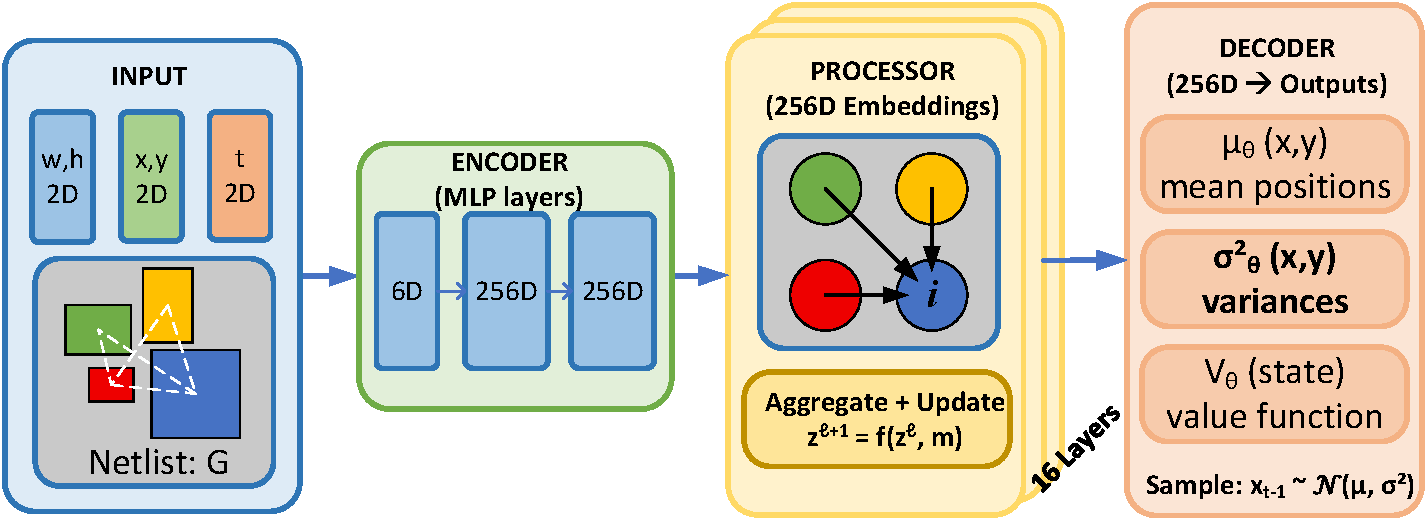
\includegraphics[width=\columnwidth]{graphs/Architecture.pdf}
\caption{The model architecture used}
\label{fig:architecture}
\end{figure}
\vspace{-10pt}  % Reduce space below

\subsection{Synthetic Training Data Generation}
\label{subsec:synthetic}

Because our method optimizes the energy function directly through policy gradients, we can generate training data efficiently without constructing near-optimal placements. We obtain synthetic datasets consisting of tuples $(\mathcal{G}, \mathbf{x}_{\text{init}})$ where $\mathcal{G}$ is a netlist and $\mathbf{x}_{\text{init}}$ represents randomized component positions.

We randomly generate components by sampling sizes from clipped exponential distributions. For each component $i$, the width and height are independently drawn from:
\begin{equation}
\label{eq:size_dist}
s_i \sim \text{ClippedExp}(\lambda_{\text{size}}, s_{\min}, s_{\max}), \quad \lambda_{\text{size}} \sim \text{Uniform}(0.04, 0.08)
\end{equation}
where $s_{\min} = 0.01$ and $s_{\max} = 1.0$. This distribution captures the characteristic heavy-tailed size distribution of real circuits, where most components are small standard cells with occasional large macros~\cite{lee2024chip}. The total component area satisfies a density constraint:
\begin{equation}
\label{eq:density}
\sum_{i=1}^N w_i h_i \leq \rho \cdot A_{\text{canvas}}, \quad \rho \sim \text{Uniform}(0.75, 0.9)
\end{equation}
where $A_{\text{canvas}} = 4$ (for the $[-1, 1] \times [-1, 1]$ normalized canvas), ensuring sufficient space for legal placements.

To generate netlists with realistic structure and to make sure each training instance does have a legal solution, we first create a temporary legal placement $\mathbf{x}_{\text{temp}}$ using collision detection, then generate three types of connections: (1) \textbf{Local proximity (60\%):} each component connects to $k_{\text{local}} \sim \text{Uniform}\{2, 4\}$ nearest neighbors via $\mathcal{N}_{\text{local}}(i) = \{j : j \in \text{TopK}(\{d_{ij}\}_{j \neq i})\}$ where $d_{ij} = \|\mathbf{x}_i^{\text{temp}} - \mathbf{x}_j^{\text{temp}}\|_1$. (2) \textbf{Hierarchical clusters (30\%):} spatial k-means partitions components into clusters ($m \sim \text{Uniform}(8, 16)$ per cluster), with inter-cluster connections weighted by $\exp(-d_{\text{cluster}}/0.5)$. (3) \textbf{Long-range (10\%):} random component pairs simulate critical paths. We merge 30\% of 2-pin nets into multi-pin nets (60\% 3-pin, 30\% 4-pin, 10\% 5-pin).

After netlist construction, component positions are randomized to create training data:
\begin{equation}
\label{eq:randomize}
\mathbf{x}_{\text{init}} = \{(x_i, y_i)\}_{i=1}^N, \quad x_i, y_i \sim \text{Uniform}(-1, 1)
\end{equation}
This destroys the spatial relationships from the temporary legal placement, creating challenging starting configurations with component overlaps and poor wirelength. During training, the model must learn to resolve these violations and optimize placement quality through policy gradient updates guided by the energy function.

We generate diverse training circuits at realistic scales: component counts $N \sim \text{Uniform}(200, 1000)$, clipped exponential size parameters $\lambda_{\text{size}} \in [0.04, 0.08]$ with bounds $[s_{\min}, s_{\max}] \in [0.01, 1.0]$, multi-scale connectivity (local + hierarchical + long-range), multi-pin nets, and canvas aspect ratios sampled from $\text{Uniform}(0.5, 2.0)$.

\subsection{Legalization Decoder}
\label{subsec:decoder}

 The trained diffusion model generates placements through reverse sampling. It produces continuous component positions that may still contain overlaps or boundary violations even with the legality penalty terms in the energy function defined in Equation~\ref{eq:energy}. To guarantee a legal placement, we employ a force-directed legalization algorithm with spatial hashing.

\begin{algorithm}[h]
\small
\caption{Force-Directed Legalization}
\label{alg:legalization}
\begin{algorithmic}[1]
\STATE Initialize uniform grid with cell size $\delta = 2 \cdot \mathbb{E}[\max(w_i, h_i)]$
\WHILE{$A_u/A_s < 0.99$ and iterations $< 1000$}
    \STATE Build spatial hash: assign each component to grid cells
    \FOR{each component $i$}
        \STATE $\mathbf{f}_i \gets \mathbf{0}$
        \FOR{each $j$ in neighboring cells of $i$}
            \IF{$i \neq j$ and $d_{ij}(\mathbf{x}) < 0$}
                \STATE $\mathbf{v}_{ij} \gets (x_j - x_i, y_j - y_i) / \|(x_j - x_i, y_j - y_i)\|$
                \STATE $\mathbf{f}_i \gets \mathbf{f}_i - |d_{ij}| \cdot \mathbf{v}_{ij}$ \COMMENT{Repulsion}
            \ENDIF
        \ENDFOR
        \IF{component $i$ outside canvas}
            \STATE $\mathbf{f}_i \gets \mathbf{f}_i - \nabla E_{\text{bound}}^{(i)}(\mathbf{x}_i)$ \COMMENT{Boundary gradient}
        \ENDIF
    \ENDFOR
    \STATE $\eta \gets \min(0.1, 1.0 / \sqrt{\text{iteration}})$ \COMMENT{Adaptive step size}
    \STATE $\mathbf{x} \gets \mathbf{x} + \eta \cdot \mathbf{f}$
\ENDWHILE
\end{algorithmic}
\end{algorithm}

The spatial hashing approach partitions the canvas into a uniform grid, allowing each component to check overlaps only with components in the same or neighboring cells. The force-directed formulation treats overlaps as repulsive forces proportional to penetration depth, while boundary violations are resolved via gradient descent on the boundary penalty $E_{\text{bound}}$. The adaptive step size $\eta$ ensures stable convergence. The algorithm converges when legality reaches $A_u / A_s \geq 0.99$ or when a maximum of 1000 iterations is reached. In practice, convergence is typically achieved in 15--30 iterations for IBM clustered circuits and 20--50 iterations for ISPD circuits, with an average of 23 iterations across all benchmarks. The legality threshold of 0.99 is chosen to ensure near-perfect legal placements while allowing minor numerical tolerances in floating-point arithmetic.

\section{Experiments}
\label{sec:experiments}

\subsection{Experimental Setup}
\label{subsec:setup}

We evaluate our energy-guided continuous diffusion approach on two standard chip placement benchmarks: ICCAD04 (IBM circuits) and ISPD2005~\cite{nam2005ispd2005}. Following ChipDiffusion~\cite{lee2024chip}, we preprocess circuits by clustering standard cells into 512 macro blocks using hMetis~\cite{karypis1999multilevel}, treating each cluster as a single component.

The training uses the Adam optimizer~\cite{kingma2015adam} with learning rate $3 \times 10^{-4}$, $\beta_1 = 0.9$, $\beta_2 = 0.999$, and $\epsilon = 10^{-8}$. We employ PPO with clipping parameter $\epsilon_{\text{clip}} = 0.2$, performing 4 PPO epochs per batch update with minibatch size of 8. The value function loss is weighted by $c_{\text{value}} = 0.5$, and gradient clipping is applied with maximum norm of 0.5. GAE parameters are $\lambda_{\text{GAE}} = 0.95$ and $\gamma = 0.99$. Training proceeds for 1000 epochs with batch size of 32 circuits, using 20,000 synthetically generated circuits with random topologies. The reward function coefficients (Eq.~\ref{eq:reward}) are $\alpha_{\text{noise}} = 0.01$ and $\alpha_{\text{ent}} = 0.001$. 1000 diffusion steps are used with cosine noise schedule $\beta_t \in [0.0001, 0.02]$, following ChipDiffusion~\cite{lee2024chip}. The energy function weights are $\lambda_{\text{overlap}} = 2.0$ and $\lambda_{\text{bound}} = 1.0$. The GNN encoder uses mean aggregation, and the value function shares the same encoder architecture with a separate MLP head. All results are reported on the average performance over five runs with different seeds. All experiments were conducted on a single NVIDIA RTX A6000 GPU paired with dual Intel Xeon Gold 5218R CPUs. Both training and inference use the same hardware configuration.

\begin{table}[h]
\centering
\caption{IBM benchmarks: HPWL averages (clustered 512, macro-only, mixed-size). Runtime for clustered.}
\label{tab:main_results}
\scriptsize
\setlength{\tabcolsep}{3pt}
\begin{tabular}{lcccc}
\toprule
Method & Clust. & Macro & Mixed & Time \\
 & ($10^7$) & ($10^5$) & ($10^6$) & (min) \\
\midrule
DREAMPlace~\cite{lin2019dreamplace} & 3.72 & -- & 23.6 & 0.48 \\
MaskPlace~\cite{lai2022maskplace} & -- & 8.72 & -- & -- \\
ChiPFormer~\cite{lai2023chipformer} & 3.15 & 7.33 & 28.9 & 124 \\
EfficientPlace~\cite{geng2024efficientplace} & -- & 8.32 & -- & -- \\
WireMask-BBO~\cite{shi2023wire} & -- & 7.43 & -- & -- \\
ChipDiffusion~\cite{lee2024chip} & 2.98 & 2.49 & 22.7 & 4.4 \\
\midrule
\textbf{Ours} & \textbf{2.84} & \textbf{2.35} & \textbf{21.8} & \textbf{4.4} \\
\bottomrule
\end{tabular}
\end{table}

\subsection{Results}
\label{subsec:main_results}

Table~\ref{tab:main_results} presents our results on IBM benchmark suite, including clustered (512-cluster preprocessing via hMetis), macro-only, and mixed-size placements. Our method achieves consistent improvements across all configurations: $2.84 \times 10^7$ on clustered benchmarks (4.6\% better than ChipDiffusion), $2.35 \times 10^5$ on macro-only (5.6\% better), and $21.8 \times 10^6$ on mixed-size (4.0\% better). For mixed-size placement, we follow ChipDiffusion's approach~\cite{lee2024chip}: using our diffusion model for macro and cluster placement, then employing DREAMPlace~\cite{lin2019dreamplace} for standard cell placement with fixed macro positions. Remarkably, our zero-shot inference on clustered benchmarks completes in 4.4 minutes on average, significantly faster than ChiPFormer (124 minutes) which requires online RL fine-tuning per circuit.

\begin{table}[h]
\centering
\caption{Detailed ISPD2005 results. HPWL ($\times 10^5$) and runtime (min). Results of the baselines are from ChipDiffusion~\cite{lee2024chip}.}
\label{tab:ispd2005}
\scriptsize
\setlength{\tabcolsep}{3pt}
\begin{tabular}{lcccccccccc}
\toprule
Circuit & \multicolumn{5}{c}{HPWL ($\times 10^5$)} & \multicolumn{4}{c}{Runtime (min)} \\
\cmidrule(lr){2-6} \cmidrule(lr){7-10}
 & MaskP. & ChiPF. & WireM. & ChipD. & Ours & MaskP. & ChiPF. & ChipD. & Ours \\
\midrule
adaptec1 & 8.57 & 6.75 & 5.81 & 9.19 & 6.1 & 139 & 223 & 4.78 & 4.8 \\
adaptec2 & 77.7 & 63.8 & 54.5 & 31.0 & 51.8 & 195 & 234 & 4.53 & 4.5 \\
adaptec3 & 108 & 73.2 & 59.2 & 54.4 & 55.2 & 224 & 284 & 4.73 & 4.7 \\
adaptec4 & 91.9 & 85.8 & 62.7 & 54.5 & 62.1 & 718 & 467 & 4.94 & 4.9 \\
bigblue1 & 3.11 & 3.05 & 2.12 & 2.64 & 2.2 & 274 & 256 & 4.83 & 4.8 \\
bigblue2 & TO & 85.8 & 186 & 38.8 & \textbf{4.5} & TO & 5220 & 122 & 121 \\
bigblue3 & 84.0 & 79.2 & 66.2 & 35.9 & 61.5 & 648 & 494 & 5.13 & 5.1 \\
bigblue4 & TO & 548 & 798 & 141 & 80.2 & TO & 1210 & 18.9 & 18.8 \\
\midrule
\textbf{Average} & -- & 116 & 154 & \textbf{45.9} & \textbf{44.2} & -- & 1049 & 21.2 & \textbf{21.1} \\
\bottomrule
\end{tabular}
\end{table}

Table~\ref{tab:ispd2005} presents detailed results on the eight ISPD2005 benchmark circuits (adaptec1-4, bigblue1-4), enabling direct comparison with recent state-of-the-art methods. We compare against MaskPlace~\cite{lai2022maskplace}, ChiPFormer~\cite{lai2023chipformer}, WireMask-BBO~\cite{shi2023wire}, and ChipDiffusion~\cite{lee2024chip}. Our method achieves an average HPWL of $44.2 \times 10^5$ across all eight circuits, competitive with ChipDiffusion's $45.9 \times 10^5$ (3.7\% improvement) and significantly outperforming ChiPFormer ($116 \times 10^5$) and WireMask-BBO ($154 \times 10^5$). Notably, MaskPlace encounters timeouts on bigblue2 and bigblue4, the two largest circuits. In terms of runtime, our approach achieves comparable efficiency to ChipDiffusion (21.1 min vs 21.2 min average), while being substantially faster than ChiPFormer (1049 min average) and WireMask-BBO (408.5 min average). This demonstrates that our unsupervised learning from synthetic data achieves strong placement quality with competitive runtime efficiency. Figure~\ref{fig:results} shows the representative placements generated by our method.

\begin{figure}[h]
\centering
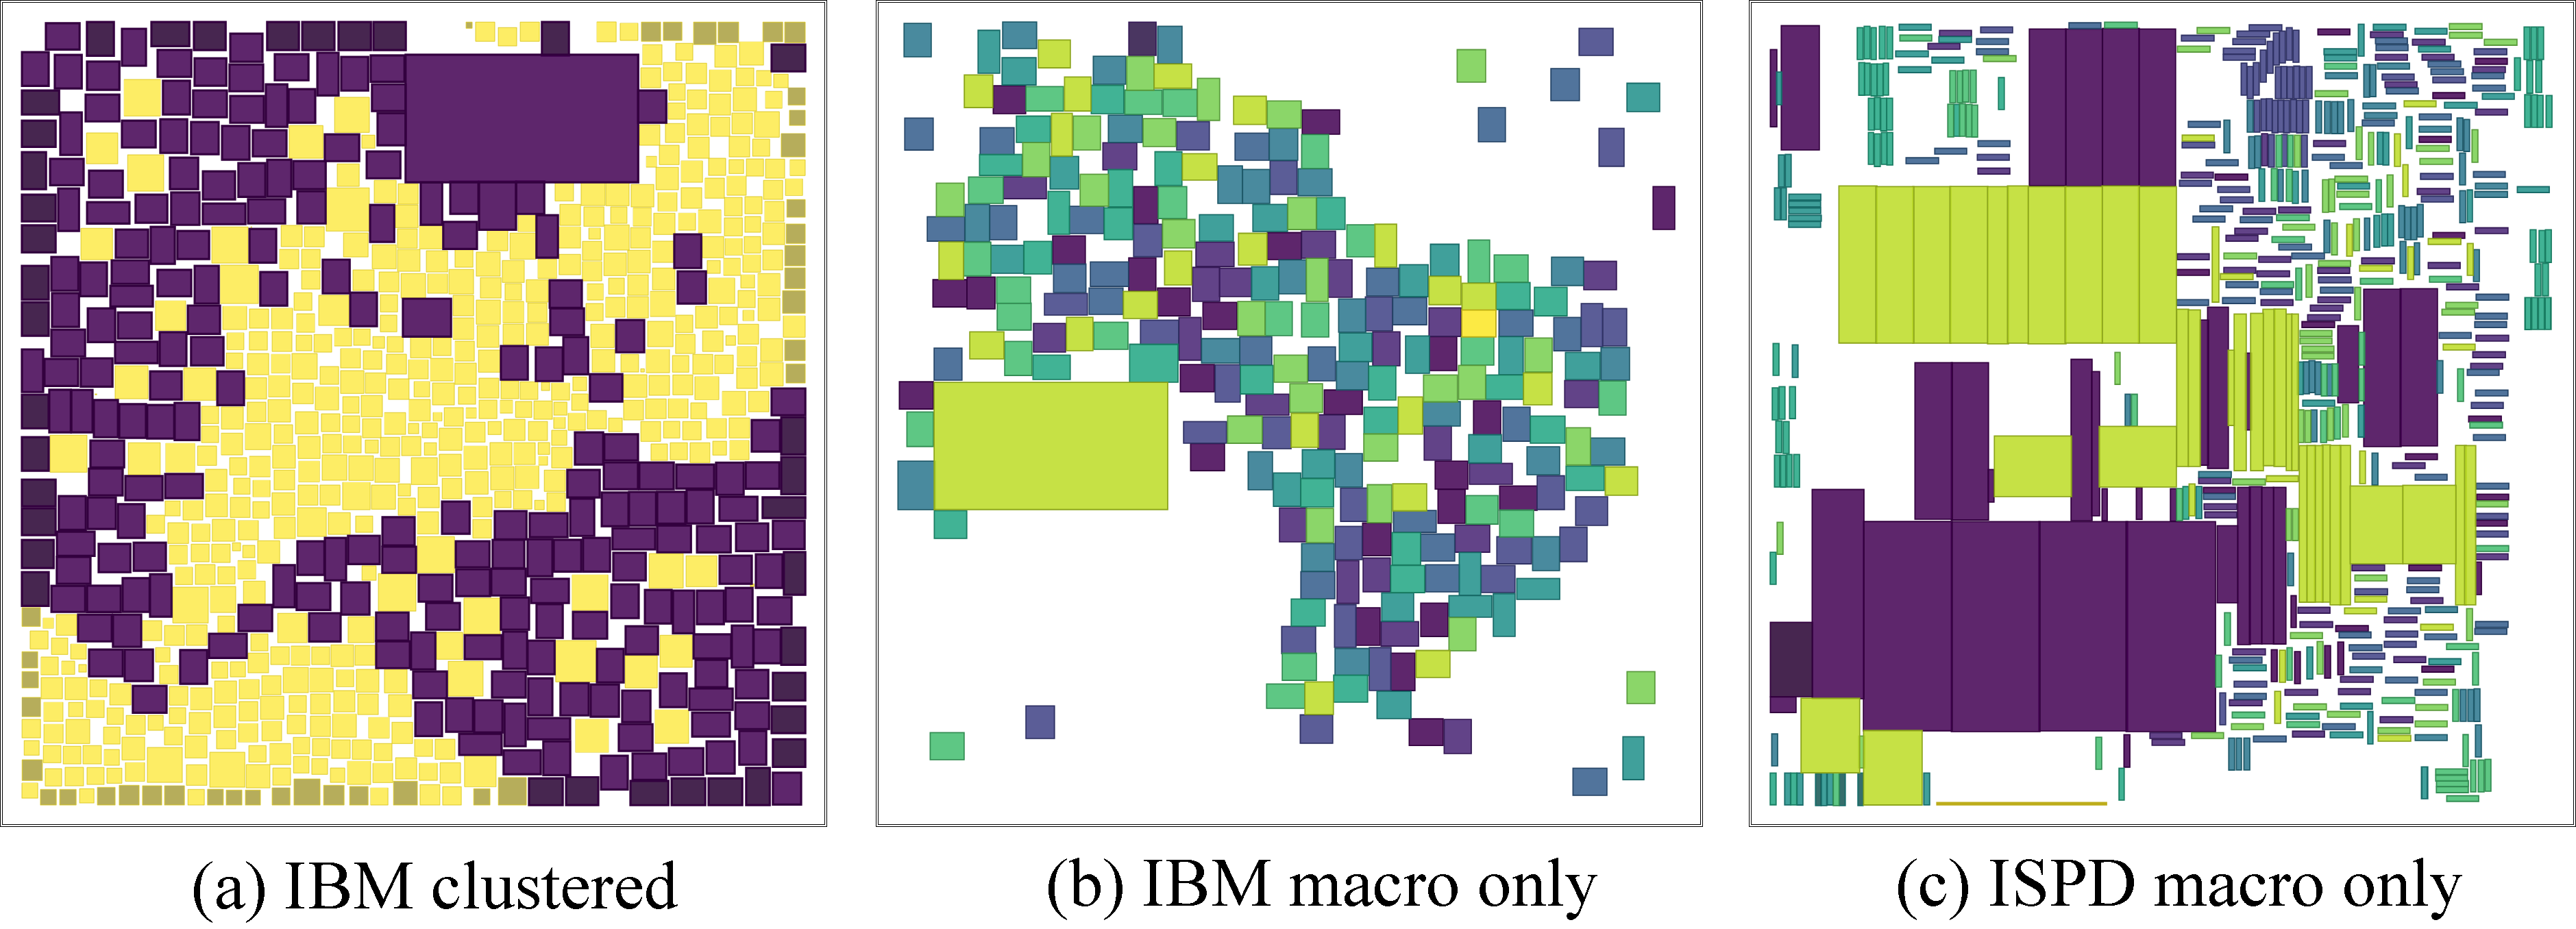
\includegraphics[width=\columnwidth]{graphs/results.pdf}
\caption{Representative placement results on (a) IBM clustered (512 clusters), (b) IBM macro-only, and (c) ISPD2005 benchmarks.}
\label{fig:results}
\end{figure}

\subsection{Ablation Studies}
\label{subsec:ablations}

\subsubsection{Dense vs. Sparse Energy Feedback} To validate the critical importance of computing energy at every diffusion time step, we compare our dense energy approach against a sparse-reward baseline that computes energy only at the final time step (similar to DDPO~\cite{black2024ddpo}). Table~\ref{tab:ablation_energy} shows that sparse energy feedback achieves only 3.42$\times 10^7$ HPWL after the same training budget, representing a 20\% degradation. Moreover, sparse training exhibits 3.2× higher gradient variance and requires 2.8× more epochs to reach comparable quality. This demonstrates that dense energy feedback substantially reduces gradient variance and accelerates convergence.

\begin{table}[h]
\centering
\caption{Dense vs. sparse energy feedback ablation.}
\label{tab:ablation_energy}
\scriptsize
\setlength{\tabcolsep}{4pt}
\begin{tabular}{lccc}
\toprule
Method & HPWL & Grad Var & Epochs \\
& ($\times 10^7$) & (relative) & to Conv. \\
\midrule
Sparse & 3.42 & 1.0× & 2800 \\
\textbf{Dense} & \textbf{2.84} & \textbf{0.31×} & \textbf{1000} \\
\bottomrule
\end{tabular}
\end{table}

\subsubsection{Legalization Decoder Contribution} We analyze the legalization decoder's impact by measuring placement quality before and after the iterative push-apart procedure (Table~\ref{tab:decoder_ablation}). Raw model outputs (before legalization) already achieve competitive HPWL with legality 0.953, while legalization increases HPWL by only 1.1\% to achieve near-perfect legality (0.9982). This minimal degradation confirms that the diffusion model learns meaningful placement structure. The decoder only enforces hard constraints. In contrast, ChipDiffusion's gradient-based legalization requires 20,000 optimization steps with carefully tuned hyperparameters (learning rates, penalty weights).

\begin{table}[h]
\centering
\caption{Decoder impact on placement quality.}
\label{tab:decoder_ablation}
\scriptsize
\setlength{\tabcolsep}{4pt}
\begin{tabular}{lcc}
\toprule
Stage & HPWL ($\times 10^7$) & Legality \\
\midrule
Raw model output & 2.81 & 0.953 \\
After legalization & 2.84 & 0.9982 \\
\midrule
HPWL degradation & \multicolumn{2}{c}{1.1\%} \\
\bottomrule
\end{tabular}
\end{table}

\subsubsection{Penalty Weight Tuning} The energy function (Equation~\ref{eq:energy}) includes penalty weights $\lambda_{\text{overlap}}$ and $\lambda_{\text{bound}}$ that balance wirelength optimization against constraint satisfaction. To determine optimal values, we conduct an empirical sweep over different weight configurations (Figure~\ref{fig:penalty_weights}). Too small weights ($\lambda_{\text{overlap}} = 0.5, \lambda_{\text{bound}} = 0.5$) lead to insufficient constraint enforcement, resulting in poor legality (0.892) despite competitive HPWL. Too large weights ($\lambda_{\text{overlap}} = 10.0, \lambda_{\text{bound}} = 5.0$) over-emphasize constraints at the expense of HPWL optimization, increasing wirelength by 8.2\% while providing minimal legality improvement beyond the 0.9982 threshold. We select $\lambda_{\text{overlap}} = 2.0$ and $\lambda_{\text{bound}} = 1.0$ as they achieve the best trade-off between HPWL and legality.

\begin{figure}[t]
\centering
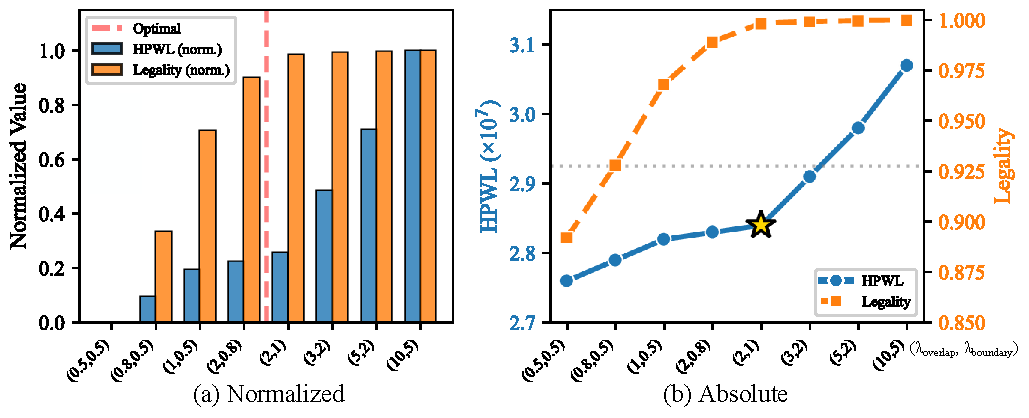
\includegraphics[width=\linewidth]{graphs/tuning.pdf}
\caption{Penalty weights tuning. (a) Normalized HPWL and legality. (b) Absolute HPWL and legality.}
\label{fig:penalty_weights}
\end{figure}

\subsubsection{Training Data Efficiency} We study how performance scales with synthetic training data size (Table~\ref{tab:data_efficiency}). Test HPWL improves logarithmically with data: training on 5K circuits achieves $3.15 \times 10^7$ HPWL, already outperforming DREAMPlace (3.724), while 20K circuits reach our best result of $2.84 \times 10^7$. This demonstrates that our method enables effective learning even from limited synthetic data, without requiring expensive real circuit placements for supervision.

\begin{table}[h]
\centering
\caption{Impact of training data size on test performance.}
\label{tab:data_efficiency}
\scriptsize
\setlength{\tabcolsep}{4pt}
\begin{tabular}{lc}
\toprule
Training Data Size & Test HPWL ($\times 10^7$) \\
\midrule
5K circuits & 3.15 \\
10K circuits & 2.94 \\
20K circuits & 2.84 \\
\midrule
\multicolumn{2}{l}{\textit{Baselines for reference:}} \\
DREAMPlace & 3.724 \\
ChipDiffusion & 2.976 \\
\bottomrule
\end{tabular}
\end{table}

\section{Conclusion and Discussion}
\label{sec:discussion}

We present a policy gradient-based diffusion model framework that enables unsupervised chip placement through direct energy optimization. By extending RL-based diffusion training from discrete to continuous domains and introducing dense per-step energy feedback, our approach addresses fundamental limitations of both supervised diffusion methods and sparse-reward reinforcement learning. Although our method is slower in inference compared to analytical placers (4.4 vs. 0.48 minutes) and the scalability to thousands of macros is unvalidated, this work still demonstrates that energy-guided policy gradient diffusion can learn effective optimization strategies purely from objective functions. This opens avenues for future work in multi-objective optimization, hierarchical decomposition for large-scale circuits, and applications to other physical design tasks such as floorplanning and global routing. 



%%
%% The next two lines define the bibliography style to be used, and
%% the bibliography file.
\newpage
\bibliographystyle{ACM-Reference-Format}
\bibliography{references}

\end{document}